\chapter{Fonctions de classe $\Cc^1$ %- Applications aux EDP
}

Soient $E$ et $F$ deux $\R$ espaces vectoriels de dimension finie munis des normes $\norm{\cdot}$ et $\norm{\cdot}'$ respectivement.

	\pl{\rep{6cm}}


\section{Définition et propriétés}

\subsection{Définition}

Soit $\U$ un ouvert d'un \rev{}  $E$ de dimension finie.
\begin{definition}
	[(Fonction de classe $\boldsymbol{\Cc^1}$)]
	Une fonction $\U \to F$ est dite de classe $\Cc^1$ si et seulement si pour tout $i=1,\cdots,n$ la fonction $\frac{\partial f}{\partial x_i}  $ est bien définie et est continue sur $\U$.
\end{definition}


\begin{exemple}
	La fonction	$f(x,y)= \begin{cases}\frac{xy}{x^2+y^2}, &\text{si $(x,y) \neq (0,0)$} \\ 0, & \text{si $(x,y) =(0,0)$ }\end{cases}$ est $\Cc^1$ sur $\R^2 \setminus \left\{ (0,0) \right\}$.
	\pl{\rep{6cm}}
\end{exemple}

%\begin{definition}
	%Soit $a,b \in E$. Le segment $[a,b]$ est l'ensemble 
	%\[
		%[a,b] = \left\{ a(1-t)+bt, t \in [0,1] \right\} \subset E.
	%\]
%\end{definition}

\subsection{Relation entre les fonctions $C^1$ et les fonctions différentiables}

\begin{theorem}
	Soit $f:E\to F$ définie sur un ouvert $\U \subset E$. On suppose que $f$ est de classe $\Cc^1$ sur $\U$. Alors $f$ est différentiable sur $\U$.
\end{theorem}

\begin{proof}
%Voir J. Royer chap4
	\pl{\rep{15cm}}
\end{proof}

\sld{\vfill\pagebreak[5]}%%%%%%%%%%%%%%%
\begin{remark}
	La réciproque est fausse: la fonction $g:\R\to\R$ définie par $g(x) =  x^2 \sin\left( \frac{1}{\abs{x}} \right) $ si $x\neq 0$ et $g(0)=0$ n'est pas $\Cc^1$ mais est différentiable sur $\R$. %Voir  Faccanoni  p.71
	\begin{center}
		\tikzexternalenable\tikzsetnextfilename{cours-nondiff}
		\begin{tikzpicture}
                    \begin{axis}[ylabel style={rotate=-90},xlabel = $x$,ylabel=$y$,zlabel=$z$,width=.45\textwidth,ymin=-.04, ymax=.04]
					%\addplot3[surf,faceted color=blue, color=blue, domain=-4:4,samples=50,opacity=.3,fill opacity=.9,id=zaza] gnuplot {(x**3+y) * exp(-x**2-y**2)};
				%\addplot3[surf,domain=-4:4,samples=50,colormap/cool,opacity=.8] gnuplot {(x**2+y**2) * sin((x**2+y**2)**(-.5) ) };
                        \addplot[blue,domain=-.2:.2,thick,samples=800,opacity=1] gnuplot {x**2 * sin( abs(x)**(-1) ) };
                                \addplot[gray,dashed,domain=-.2:.2,samples=50,opacity=.5] {x^2};
                                \addplot[gray,dashed,domain=-.2:.2,samples=50,opacity=.5] {-x^2};
			\end{axis}
		\end{tikzpicture}
		\tikzexternaldisable
	\end{center}
	\pl{\rep{4cm}}
\end{remark}


%\sld{\vfill\pagebreak[5]}%%%%%%%%%%%%%%%
%On note $\mathcal L(E,F)$ l'espace vectoriel des applications linéaires de $E$ dans $F$ que l'on munit de la norme 
%\[
	%\tnorm{\ell} = \sup_{x\in E \setminus \left\{ 0 \right\}} \frac{\norm{\ell(x)}'}{\norm{x}}
%\]
%pour tout $\ell \in \mathcal L(E,F)$.
%\begin{proposition}
	%Soit $f:\U\to F$. Les propositions suivantes sont équivalentes:
	%\begin{enumerate}
		%\item $f$ est de classe $\Cc^1$ sur $\U$
		%\item Pour tout $a\in\U$, $f$ est différentiable en $a$ et l'application (définie sur $\U$) \begin{align*} df: (E,\snorm{\cdot}) & \to (\mathcal L(E,F),\tnorm{\cdot}) \\a &\mapsto d_a f\end{align*} est continue sur $\U$. L'application $df$ est appelée \emph{différentielle} de $f$.
	%\end{enumerate}
%\end{proposition}

%\begin{proof}
	%Admis bien que ce soit un corollaire du théorème précédent.
%\end{proof}
 
%\begin{remark}
%Lorsque $f\in \Cc^1(\U,F)$ alors $df \in \Cc^0(\U,\mathcal L(E,F))$.	
%\end{remark}

%\sld{\vfill\pagebreak[5]}%%%%%%%%%%%%%%%


%\subsection{Inégalité des accroissements finis}

%\begin{theorem}
	%[(Inégalité des accroissements finis)] 
	%Soit $\U$ un ouvert de $E$ et $f: \U \to F$ une fonction différentiable sur $\U$. On considère deux points $a$ et $b$ de $\U$ tels que $[a,b] \subset \U$ et on suppose qu'il existe $M \geq 0$ tel que pour tout $x\in [a,b]$:
	%\[
		%\tnorm{d_x f} \leq M
	%\]
	%Alors 
	%\[
		%\norm{f(b) - f(a)}' \leq M \norm{b-a}
	%\]
%\end{theorem}

%\begin{proof}
%Admis.%(Denizeau p22 et p8).
%\end{proof}

\sld{\vfill\pagebreak[5]}%%%%%%%%%%%%%%%
\section{Composition des fonctions de classe $\Cc^1$}

	Soient $E,F,G$ trois espaces vectoriels normés de dimension finie.

	\begin{theorem}[(Règle de la chaine)]
Soient $f:E \to F$ une application de classe $\Cc^1$ sur l'ouvert $\U \subset E$ et $g:F\to G$ une application de classe $\Cc^1$ sur l'ouvert $\V\supset f(\U)$. Alors $g\circ f: E\to G$ est de classe $\Cc^1$ sur $\U$ avec, pour tout $x\in U$:
	\[
		d_x (g\circ f) = d_{f(x)} g\circ d_x f 
	\]
\end{theorem}

\begin{proof}
	\plprof{Idée de la preuve (voir Denizeau p 20)}
	\pl{\rep{10cm}}
\end{proof}

\begin{remark}
	Il s'agit de la généralisation de la formule de dérivation d'une composée pour $f,g:\R\to\R$. On a alors pour $x\in\R$ $(g\circ f)'(x) = g'(f(x)) f'(x)$.
\end{remark}

\sld{\vfill\pagebreak[5]}%%%%%%%%%%%%%%%
\begin{proposition}
	Soient $f:E \to F$ une application de classe $\Cc^1$ sur l'ouvert $\U \subset E$ et $g:F\to G$ une application de classe $\Cc^1$ sur l'ouvert $\V\supset f(\U)$.
	
	La matrice jacobienne de $g\circ f$ en $x\in\U$ est donnée par 
	\[
		J_{\gf} (x) = J_{g}(f(x)) \cdot J_f(x).
	\]
\end{proposition}

\begin{proof}
	C'est la traduction matricielle du théorème précédent.
\end{proof}

\sld{\vfill\pagebreak[5]}%%%%%%%%%%%%%%%
On note $\mathcal B = (e_1,\cdots,e_n)$ une base de $E$ et $\mathcal B' = (e'_1,\cdots,e'_p)$ une base de $F$. Soit une application $f:E \to F$, on note $f_1,\cdots,f_p: E \to \R$ les fonctions coordonnées de $f$ dans la base $\mathcal B'$. Autrement dit, on a $f(x) = f_1(x) e'_1 + \cdots + f_p(x) e'_p \in F$  pour tout $x\in E$.
\begin{proposition}
	Soient $f:E \to F$ une application de classe $\Cc^1$ sur l'ouvert $\U \subset E$ et $g:F\to \R$ une application de classe $\Cc^1$ sur l'ouvert $\V\supset f(\U)$.
	Alors en tout point $(x_1,\cdots,x_n) \in \U$, on a pour tout $j = 1,\cdots,n $
	\[
		\frac{\partial \gf}{\partial x_j}(x_1,\cdots,x_n) = \sum_{i=1}^p \frac{\partial g}{\partial f_i}(f_1(x) , \cdots, f_p(x) ) \frac{\partial f_i}{\partial x_j}(x_1,\cdots,x_n).
	\]
	où on a noté $ \frac{\partial g}{\partial f_i}(f_1(x) , \cdots, f_p(x) )$ la $i$-ème dérivée partielle de $g$ en $f(x) \in \V$.
\end{proposition}

\begin{proof}
	\pl{\rep{6cm}}
\end{proof}

\sld{\vfill\pagebreak[5]}%%%%%%%%%%%%%%%
\begin{remark}
	%Le produit matriciel ci dessus est bien défini. On a  $ J_{g}(f(a))$  $\cdot J_f(a)$ 
	On a la notation plus condensée suivante: 
	\[
		\frac{\partial \gf}{\partial x_j} = \sum_{i=1}^p \frac{\partial g}{\partial f_i} \frac{\partial f_i}{\partial x_j}.
	\]
	La formule est concise mais les abus de notations peuvent être trompeurs pour le néophyte\ldots
\end{remark}


%Application et exemple de J. Royer
\begin{exemple}
	Coordonnées cylindriques~: $\psi(r,\theta) = (r\cos(\theta), r \sin(\theta))$ et $f:\R^2 \to \R$ de classe $\Cc^1$ sur $\R^2$. Calcul de $\frac{\partial f \circ \psi}{\partial x_j}$.
	\pl{\rep{6cm}}
\end{exemple}

\sld{\vfill\pagebreak[5]}%%%%%%%%%%%%%%%

\section{Difféomorphismes}

Soient $E$ et $F$ deux $\R$ espaces vectoriels normés de dimension finie et $\U$ et $\V$ deux ouverts de $E$ et $F$ respectivement. %Soit $k\in \N\setminus \left\{ 0 \right\}$.
\begin{definition}[(Difféomorphismes)]
 	On dit que $f$ est un $\Cc^1$-difféomorphisme de $\U$ vers $\V$ si $f$ est une bijection de classe $\Cc^1$ de $\U$ sur $\V$  dont la réciproque $f^{-1}$ est de classe $\Cc^1$ sur $\V$.
\end{definition}

\begin{exemple}
	L'application $(x,y) \mapsto (x+y,x-y)$ est un $\Cc^1$-difféomorphisme de $\R^2$ dans $\R^2$.
\end{exemple}
%\begin{exemple}
	%L'application $(x,y) \mapsto (xy,\frac y x)$ es un $\Cc^\infty$-difféomorphisme de $(\R)^2$ dans $\R^2$.
%\end{exemple}
\begin{exemple}
	L'application $\phi: x\mapsto \operatorname{Sign}(x) \sqrt{\abs{x}} $ est une bijection de $\R$ dans $\R$ d'inverse $\phi^{-1}: x \mapsto \operatorname{Sign}(x) x^2$. L'application $\phi^{-1}$ est $\Cc^1$ sur $\R$ mais $\phi$ n'est pas $\Cc^1$.
	\pl{\rep{6cm}}
\end{exemple}

\sld{\vfill\pagebreak[5]}%%%%%%%%%%%%%%%
\begin{proposition}
	Soit $f:E\to F$ un $\Cc^1$ difféomorphisme de $\U$ sur $\V$. Alors pour tout $a\in \U$, $d_a f$ est un isomorphisme de $E$ sur $F$ tel que 
	\[
		(d_a f)^{-1} = d_{f(a)} (f^{-1}).
	\]
\end{proposition}

\begin{proof}
	\pl{\rep{3cm}}
\end{proof}

\begin{remark}
	On a donc $\dim E = \dim F $.
\end{remark}

On dispose de la caractérisation suivante des difféomorphismes
\begin{theorem}
	[(Inversion globale)] Soit $\U$ un ouvert de $E$ et $f:\U \to F$ une application injective de classe $\Cc^1$. Alors $f$ définit un $\Cc^1$ difféomorphisme du $\U$ sur $f(\U)$ si et seulement si $d_a f$ est un isomorphisme pour tout $a\in\U$.
\end{theorem}

\begin{proof}
	Admis.
\end{proof}

\sld{\vfill\pagebreak[5]}%%%%%%%%%%%%%%%
\begin{remark}
	\pl{\rep{4cm}}
\end{remark}

\begin{exemple}
Coordonnées polaires: $\psi(r,\theta) = (r\cos(\theta), r \sin(\theta))$ est un $\Cc^1$-difféomorphisme de  $ ]0,+\infty[ \times ]-\pi , \pi[$ dans $\R^2 \setminus ( \R^- \times \left\{ 0 \right\}) $ ($\R^2$ privé de la demi-droite des réels négatif).
	\pl{\rep{6cm}}
\end{exemple}

\sld{\vfill\pagebreak[6]}%%%%%%%%%%%%%%%
\section{Fonctions implicites}

Dans $\R^2$, la droite $\D$ d'équation 
\[
ax + by +c = 0
\]
est la ligne de niveau 0 de la fonction $(x,y) \mapsto ax +by +c$. Si $b \neq 0$ (\ie si la droite n'est pas verticale) on peut définir la fonction $\varphi(x) = -\frac{ax+c}{b}$ de sorte que $(x,\varphi(x)) \in \D$ pour tout $x\in\R$. De la même manière, si $a \neq 0$ les points $(\phi(y),y) $ où $\phi(y) =-\frac{by+c}{a}$ sont sur $\D$. 

\begin{center}
    \tikzsetnextfilename{coursImplicit}
    \begin{tikzpicture}
        \begin{axis}[axis x line=middle,
                     axis y line=middle,
                     xlabel = {$x$},
                     every axis x label/.style={at={(current axis.right of origin)},anchor=north west},
                     ylabel = {$y$},
                     every axis y label/.style={at={(current axis.above origin)},anchor=north east},
                     enlargelimits,
                   %  ymin=-6,ymax=6,xmin=-4,xmax=6,
                     after end axis/.code = {
                         \draw[red] (axis cs:-3.1,0) -- (axis cs:3.1,0);
                         \draw[green!50!black] (axis cs:0,-2.1) -- (axis cs:0,4.1);
                     }
                    ]				
                     \addplot[color=blue,id=excurve1,domain=-3:3,smooth,samples=10, very thick] gnuplot {x+1} node[rotate=-90,green!50!black, pos=.3, above=4em]{$x=y-1$} node[red, pos=.6, below right]{$y=x+1$};
        \end{axis}
    \end{tikzpicture}
\end{center}


\begin{remark}
    En physique, on utilise très souvent cette formulation implicite. Par exemple, la loi d'Ohm, souvent énoncée par $U=RI$, devrait plutôt être comprise comme la formulation implicite de la courbe de niveau $0$ de l'application  $f(U, R, I) = U - RI$. En effet, on peut, suivant les besoins, exprimer $U$ en fonction de $R$ et de $I$, ou $I$ en fonction de $U$ et de $R$, \textit{etc}\ldots 
\end{remark}

\medskip

{\bf\sffamily Question:} étant donnée une équation $f(x,y) =0$. À quelles conditions sur $f$ peut-on faire le même procédé ?

\sld{\vfill\pagebreak[5]}%%%%%%%%%%%%%%%
\begin{definition}
Soit $f:\R^2 \to \R$ et $T=\left\{ (x,y) \in\R^2 | f(x,y) = 0 \right\}$. Si $T$ peut être représenté au voisinage de $ (x_0,y_0) \in T$ par le graphe d'une fonction $\varphi:]a,b[\to \R $ où $x_0 \in ]a,b[$ (\ie $(x,\varphi(x)) \in T $ pour tout $x\in]a,b[$), alors on dit que $\varphi$ est une fonction implicite de l'équation $f(x,y) =0$.
\end{definition}

\begin{exemple}
        Soit $f(x,y) = x^2 + y^2 -1$. 
        \pl{\rep{7cm}}
\end{exemple}

\sld{\vfill\pagebreak[5]}%%%%%%%%%%%%%%%
\begin{theorem}[(Fonction implicite sur $\R^2$)]
        Soit $f:\U \to \R$ une fonction de classe $\Cc^1$ sur $\U$ ouvert de $\R^2$ et $(x_0,y_0) \in \U $. Si $f(x_0,y_0) = 0$ et $\frac{\partial f}{\partial y} (x_0,y_0)  \neq 0$ alors il existe un intervalle ouvert $I$ contentant $x_0$ et une unique fonction $\varphi:I \to \R$ de classe $\Cc^1$ telle que:
        \begin{enumerate}
                \item $\varphi(x_0) = y_0$.
                \item $f(x,\varphi(x)) = 0$ pour tout $x\in I$.
                \item $\varphi'(x) = -\frac{\frac{\partial f}{\partial x} (x,\varphi(x))  }{\frac{\partial f}{\partial y} (x,\varphi(x)) }$ pour tout $x\in I$.
                \item la droite tangente à la courbe $y=\varphi(x)$ en $x=x_0$ a pour équation $y=\varphi'(x_0) (x-x_0) + y_0 $.
        \end{enumerate}
\end{theorem}

\begin{proof}
        Admis. Mais on trouvera une preuve dans \cite{LM} page 204.
\end{proof}

\sld{\vfill\pagebreak[5]}%%%%%%%%%%%%%%%
\begin{exemple}
        Soit $f:\R^2 \to \R$ définie par $f(x,y) = y^2 - y -3x$  et le point $(x_0,y_0) = (2,-2)$. On a $f(2,-2) = 0$ et on considère la courbe de niveau 0.

        \begin{center}
%		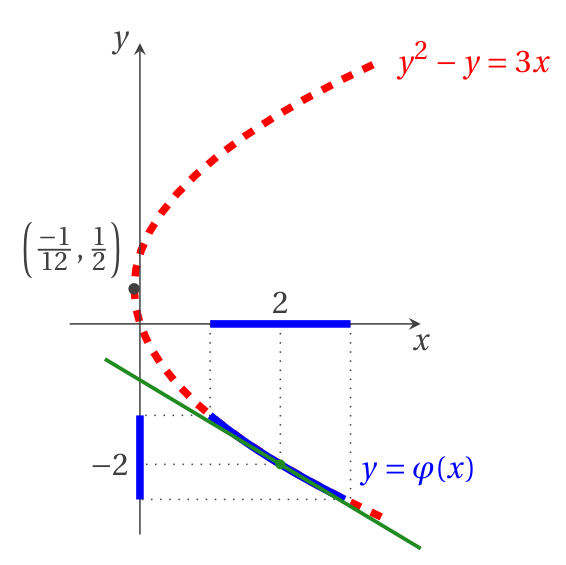
\includegraphics[height=5cm]{./figures/fonctionsImplicites.png}
                \tikzexternalenable \tikzsetnextfilename{cours-fimp}
                \begin{tikzpicture}
                        \begin{axis}[x post scale=1,
                                        axis lines = center,
                                        xmin=-.5,
                                        xmax=3.2,
                                        xlabel = {$x$},
                                        every axis x label/.style={at={(current axis.right of origin)},anchor=north west},
                                        ylabel = {$y$},
                                        every axis y label/.style={at={(current axis.above origin)},anchor=north east},
                                        xticklabels={},
                                        extra x ticks={2},
                                        extra x tick labels={$2$},
                                        extra x tick style={  xticklabel style={yshift=0.5ex, anchor=south}},
                                        after end axis/.code={% add labels
                                        \draw (axis cs: -1/12,.5) node[left] {\tiny $(-\tfrac{1}{12} , \tfrac 1 2 )$} circle (1pt);%
                                        \node[below right] at (aa) {$ y^2 - y =3x $};
                                        \node[above right,blue] at (bb) {$y = \varphi(x)$};
                                }]

                                \draw[gray,dashed] (2,0) -- (2,-2) -- (0,-2) ;
                                \draw[gray,dashed] (1.53,0) -- (1.53,-1.7) -- (0,-1.7) ;
                                \draw[gray,dashed] (2.53,0) -- (2.53,-2.3) -- (0,-2.3) ;
                                
                                \addplot[very thick, blue!40, domain=-2.5:.5, samples=100] ({(x^2 -x ) /3},{x}) node[pos=.9] (aa) {};	
                                \addplot[very thick, red!40, domain=.5:3.5, samples=100] ({(x^2 -x ) /3},{x}) node[pos=.9] (aa) {};	
                                %plot tangente
                                %\draw[green] (0,-.8) -- (2,-2) ;
                                \addplot[green!50!black, very thick, domain=-.5:3] {-3/5 * x -.8 } ;

                                % plot fonction implicites
                                \draw[blue] (0,-1.7) -- (0,-2.3) ;
                                \draw[blue] (1.53,.0) -- (2.53,0) ;
                                \addplot[very thick, blue, domain=-1.7:-2.3] ({(x^2 -x ) /3},{x}) node[pos=1] (bb) {};

                                

                        \end{axis}
                \end{tikzpicture}
        \end{center}
        \pl{\rep{7cm}}
\end{exemple}


